\subsection{Bestimmung der Dichten der Stäbe}

\subsubsection{Eckiger Stab}
Der Mittelwert der $N=\SI{10}{}$ gemessenen Breiten $d_{e}$ (Tab. \ref{tab:breiten}) des eckigen Stabs errechnet sich durch:
\begin{equation}
  \mu_{e} = \frac{1}{N} \sum_{n=1}^{N} d_{e, n}
  \label{eqn:emu}
\end{equation}
und wird als
\begin{equation*}
  \mu_{e}= \SI{0.01012}{m}
\end{equation*}
errechnet.
Die zugehörige Standardabweichung wird mithilfe der folgenden Formel ermittelt:
\begin{equation}
  \sigma_{e} =  \sqrt{  \frac{1}{N-1}  \sum_{n=1}^{N} (d_{e, n} - \mu_{e})^2 }
  \label{eqn:esigma}
\end{equation}
und ergibt sich als
\begin{equation*}
  \sigma_{e}= \SI{1.32665e-4}{m}.
\end{equation*}
Die Varianz wird folgendermaßen ermittelt:
\begin{equation}
  V_{e}= \frac{\sigma_{e}}{\sqrt{N}}.
  \label{eqn:evar}
\end{equation}
Die Varianz ist
\begin{equation*}
  V_{e}= \SI{0.000042}{m}.
\end{equation*}
Somit ergibt sich als verwendete Breite des eckigen Stabes
\begin{equation*}
  a=\SI{0.01012 \pm 0.000042}{m}.
\end{equation*}
Das Volumen des eckigen Stabs wird daraufhin mit
\begin{equation}
  Vol_{e}=a^2 \cdot l_{e}
  \label{eqn:evol}
\end{equation}
errechnet und ergibt mit $l_{e}= \SI{0.6}{m}$:
\begin{equation*}
  {Vol}_{e}= \SI{0.000614486 \pm 0.00000000106}{m^3}.
\end{equation*}
Die Dichte des eckigen Stabs wird dann mit $m_{e}=\SI{0.5024}{kg}$ mit folgender Formel ermittelt:
\begin{equation}
  \rho_{e}= \frac{m_{e}}{Vol_{e}}.
  \label{eqn:erho}
\end{equation}
Die Dichte wird als
\begin{equation*}
  \rho_{e}=\SI{8175.93359 \pm 0.14050}{\frac{kg}{m^3}}
\end{equation*}
bestimmt.


\subsubsection{Runder Stab}
Der Mittelwert der zehn gemessenen Radien $d_{r}$ (Tabelle \ref{tab:breiten}) des runden Stabs wird durch Gleichung \eqref{eqn:emu} ermittelt und ergibt sich zu
\begin{equation*}
  \mu_{r}=\SI{0.0049975}{m}.
\end{equation*}
\begin{table}[h]
  \centering
  \caption{Messdaten: Abmessungen der Stäbe}
  \label{tab:tabBreiten}
  \begin{tabular}{c c}
    \toprule
     $d_{e}/m$	&  $d_{r}/m$	 \\
    \midrule
      \begin{table}[h]
  \centering
  \caption{Messdaten: Abmessungen der Stäbe}
  \label{tab:tabBreiten}
  \begin{tabular}{c c}
    \toprule
     $d_{e}/m$	&  $d_{r}/m$	 \\
    \midrule
      \begin{table}[h]
  \centering
  \caption{Messdaten: Abmessungen der Stäbe}
  \label{tab:tabBreiten}
  \begin{tabular}{c c}
    \toprule
     $d_{e}/m$	&  $d_{r}/m$	 \\
    \midrule
      \input{tabBreiten.txt}
    \bottomrule
  \end{tabular}
\end{table}

    \bottomrule
  \end{tabular}
\end{table}

    \bottomrule
  \end{tabular}
\end{table}

Die entsprechende Standardabweichung wird folgendermaßen nach Gleichung \eqref{eqn:esigma} errechnet.
Die Standardabweichung wird als
\begin{equation*}
  \sigma_{r}=\SI{0.0000075}{m}
\end{equation*}
errechnet.
 Die Varianz wird nach Gleichung \eqref{eqn:evar} ermittelt.
 Die Varianz für den runden Stab ist
\begin{equation*}
  V_{r}=\SI{0.00000237}{m}.
\end{equation*}
 Der verwendete Radius des runden Stabs beläuft sich entsprechend auf
\begin{equation*}
  r=\SI{0.0049975 \pm 0.00000237}{m}.
\end{equation*}
 Der runde Stab hat ein Volumen, das über Gleichung \eqref{eqn:evol} berechnet wird
 und sich mit $l_{r}=\SI{0.55}{m}$ als
\begin{equation*}
  {Vol}_{r}= \SI{0.0000432 \pm 0.000000000000972}{m^3}
\end{equation*}
 ergibt.
 Die Dichte des runden Stabs wird unter Nutzung von $m_{r}=\SI{0.3605}{kg}$ mit Gleichung \eqref{eqn:erho} errechnet:
\begin{equation*}
  \rho_{r}=\SI{8353.8582 \pm 0.0019}{\frac{kg}{m^3}}.
\end{equation*}

\subsection{Bestimmung der Durchbiegung D(x)}
Zunächst werden die y-Werte der Messreihen von den jeweiligen Nullmessungen abgezogen um die entsprechenden Werte D(x) zu erhalten.
\begin{equation}
  D(x)=y_{Nullmessung} - y_{Messreihe}
  \label{eqn:durchbiegung}
\end{equation}
 Die Funktionen für die jeweiligen Elastizitätsmodule werden in Hilfsfunktionen zerlegt.
 Für das Elastizitätmodul des eckigen Stabs bei der einseitigen Einspannung wird die Hilfsfunktion
\begin{equation}
  g_{e}(x) = l_{e} \cdot x^2 - \frac{x^3}{3}
  \label{eqn:ge}
\end{equation}
 definiert.
 Die Hilfsfunktion des Elastizitätsmoduls des runden Stabs bei der einseitigen Einspannung lautet:
\begin{equation}
  g_{r}(x) = l_{r} \cdot x^2 - \frac{x^3}{3}
  \label{eqn:gr}
\end{equation}
 Für die beidseitige Einspannung sind zwei verschiedene Hilfsfunktionen erforderlich.
\begin{equation}
  g_{br}(x) = 3 l_{e}^2 \cdot x - 4 x^3
  \label{eqn:grechts}
\end{equation}
 gilt für den Bereich $\frac{l_{e}}{2} \geq x \geq 0$, während
\begin{equation}
  g_{bl}(x) =  4 x^3 - 12 l_{e} \cdot x^2 + 9 l_{e}^2 \cdot x - l_{e}^3
  \label{eqn:grechts}
\end{equation}
 für den Bereich $l_{e} \geq x \geq \frac{l_{e}}{2}$ gilt.
 Nun werden die Werte von D(x) gegen die Werte von g(x) für den einseitig eingespannten eckigen Stab,
für den einseitig eingespannten runden Stab, für die rechte Seite ($\frac{l_{e}}{2} \geq x \geq 0$) des beidseitig eingespannten eckigen Stab und für die linke Seite ($l_{e} \geq x \geq \frac{l_{e}}{2}$) des beidseitig eingespannten eckigen Stab aufgetragen.
 Die verwendete Formel für die lineare Regression lautet
\begin{equation*}
  y= n \cdot x+b.
  \label{eqn:linreg}
\end{equation*}

\begin{figure}[h!]
  \centering
  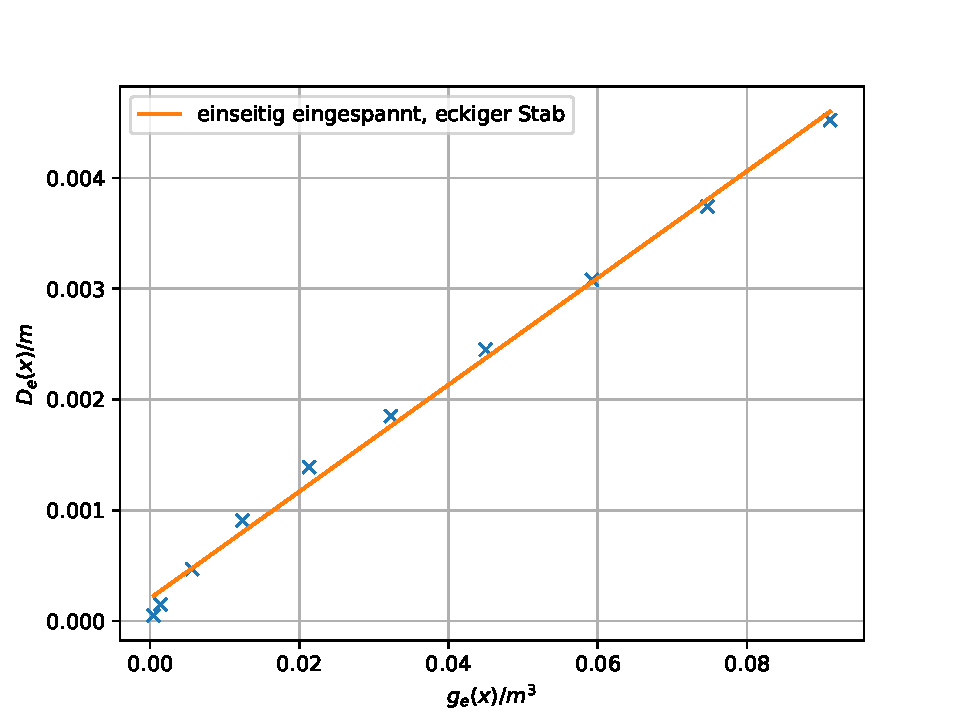
\includegraphics[width=\textwidth]{plotdge.pdf}
  \caption{$g_{e}(x)$ gegen $D_{e}(x)$}
  \label{fig:dge}
\end{figure}

\begin{figure}[h!]
  \centering
  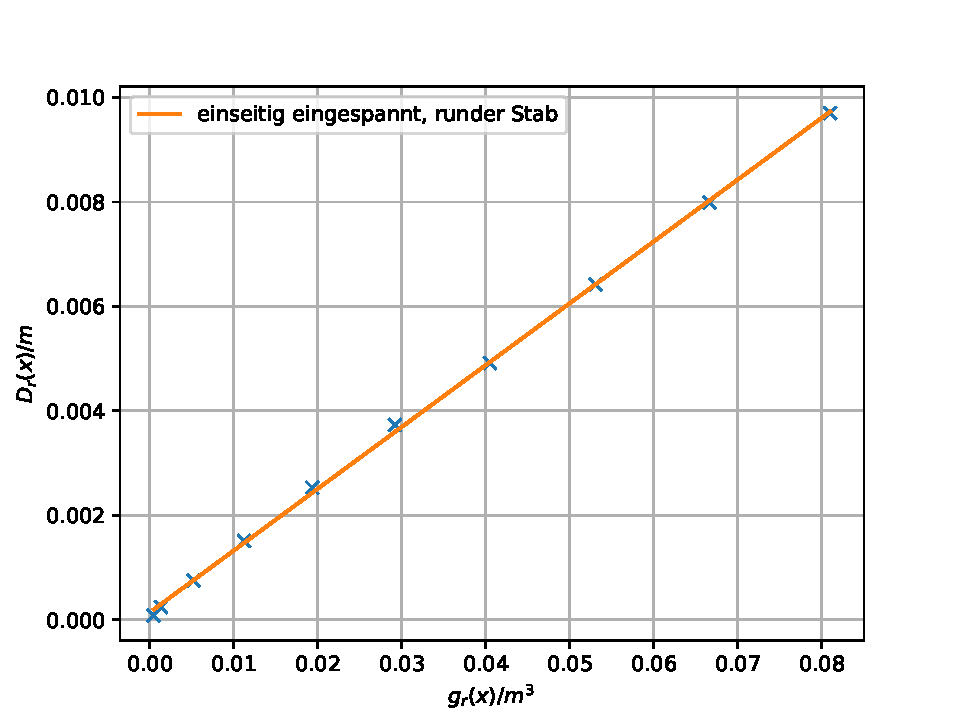
\includegraphics[width=\textwidth]{plotdgr.pdf}
  \caption{$g_{r}(x)$ gegen $D_{r}(x)$}
  \label{fig:dgr}
\end{figure}

\begin{figure}[h!]
  \centering
  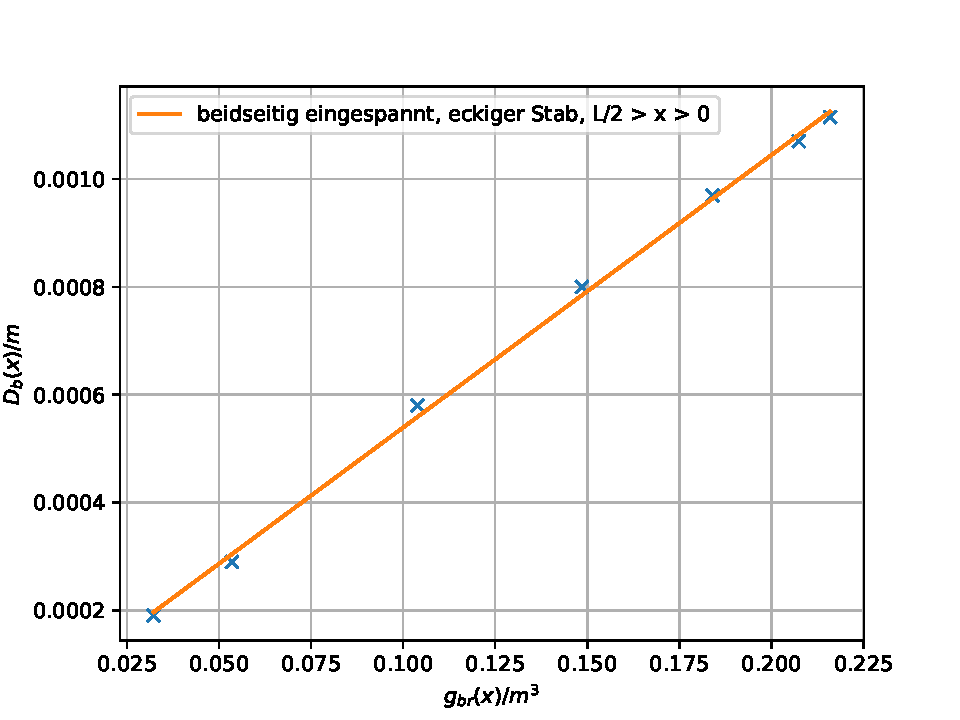
\includegraphics[width=\textwidth]{plotdgbr.pdf}
  \caption{$g_{br}(x)$ gegen $D_{br}(x)$}
  \label{fig:dgbr}
\end{figure}

\begin{figure}[h!]
  \centering
  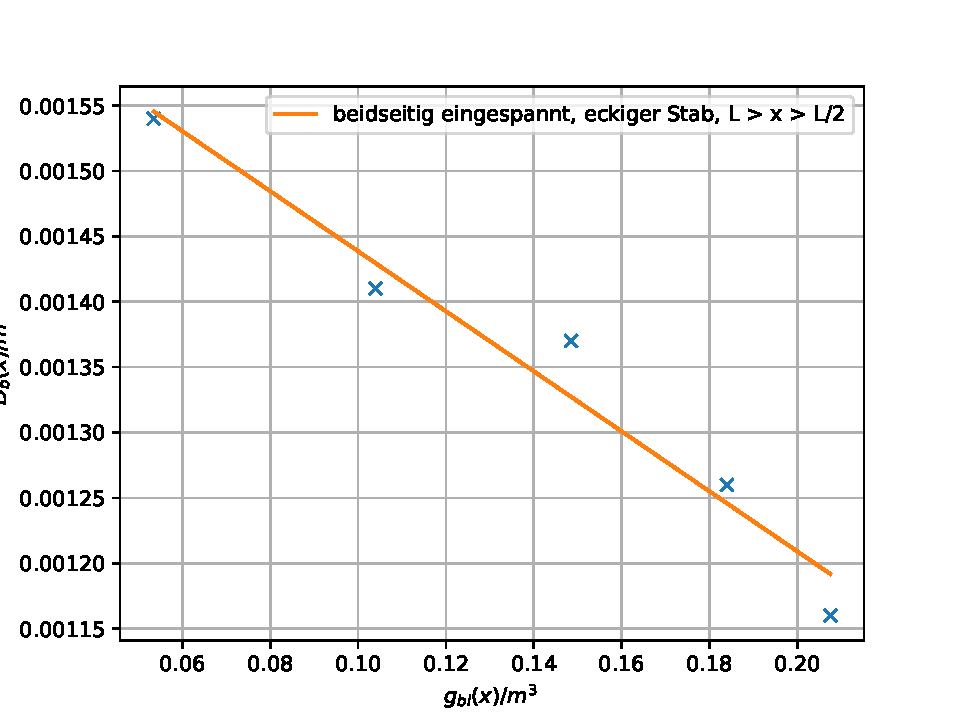
\includegraphics[width=\textwidth]{plotdgbl.pdf}
  \caption{$g_{bl}(x)$ gegen $D_{bl}(x)$}
  \label{fig:dgbl}
\end{figure}

\begin{landscape}
  \begin{table}
  \centering
  \caption{Messdaten: Breiten der Stäbe}
  \label{tab:breiten}
  \begin{tabular}{c c c c c c c c}
    \toprule
    x/m & $D_{e}(x)/mm$	& $g_{e}(x)/m^3$ & $D_{r}(x)/mm$ & $g_{r}(x)/m^3$ & $D_{b}(x)/mm$ & $g_{br}(x)/m^3$ & $g_{bl}(x)/m^3$  \\
    \midrule
      \input{D(x).txt}
    \bottomrule
  \end{tabular}
\end{table}

\end{landscape}

Die Parameter der einzelnen linearen Regressionen werden mittels Python bestimmt und lauten:
\begin{align*}
  n_{e}  &=& \SI{0.04823 \pm 1.465e-06}{m^{-2}}\\
  b_{e}  &=& \SI{0.00020 \pm 3.091e-09}{m}\\
  &&(Abb. \ref{fig:dge})
   & \\
  n_{r}  &=& \SI{0.11837 \pm 8.652e-07}{m^{-2}}\\
  b_{r}  &=& \SI{0.00014 \pm 1.457e-09}{m}\\
  &&(Abb. \ref{fig:dgr})
   &  \\
  n_{br} &=& \SI{0.00505 \pm 7.524e-09}{m^{-2}}\\
  b_{br} &=& \SI{0.00003 \pm 1.723e-10}{m}\\
  &&(Abb. \ref{fig:dgbr})
   &  \\
  n_{bl} &=& \SI{-0.00230 \pm 7.490e-08}{m^{-2}}\\
  b_{bl} &=& \SI{ 0.00167 \pm 1.687e-09}{m}\\
  &&(Abb. \ref{fig:dgbl})
   &  \\
\end{align*}

\subsection{Bestimmung des Elastizitätmoduls E bei einseitiger Einspannung}
Die Flächenträgheitsmomente berechneten sich aus
\begin{equation}
  I_{e}= \frac{a^4}{12}
  \label{eqn:ie}
\end{equation}
 und
\begin{equation}
  I_{r}= \frac{\pi \cdot r^4}{4}.
  \label{eqn:ir}
\end{equation}
 Die Fehler errechnen sich über die Gauß'sche Fehlerfortpflanzung:
\begin{align*}
  \Delta I_{e} &=& \sqrt{ \left(\frac{d I_{e}}{da}\right)^2 \cdot \left(\Delta a \right)^2 } \\
  \Delta I_{r} &=& \sqrt{ \left(\frac{d I_{r}}{dr}\right)^2 \cdot \left(\Delta r \right)^2 } \\
\end{align*}
 Für den eckigen Stab ergibt sich
\begin{equation*}
  I_{e}=\SI{8.74405 \pm 0.14499e-10}{m^4}.
\end{equation*}
 Das Flächenträgheitsmoment des runden Stabs beläuft sich auf
\begin{equation*}
  I_{r}= \SI{4.89893 \pm 0.00930e-10}{m^4}.
\end{equation*}

\subsubsection{Eckiger Stab}
Das Elastizitätsmodul des eckigen Stabs berechnete sich aus:
\begin{equation}
  E_{e} = \frac{m_{g} \cdot g}{2 \cdot I_{e}} \cdot \frac{g_{e}(x)}{D_{e}(x)} = \frac{m_{g} \cdot g}{2 \cdot I_{e}} \cdot \frac{1}{n_{e}}.
  \label{eqn:eela}
\end{equation}
 Der Fehler für $E_{e}$ wird durch die Gauß'sche Fehlerfortpflanzung bestimmt:
\begin{equation}
    \Delta E_{e} = \sqrt{ \left(\frac{d E_{e}}{d I_{e}} \right)^2 \cdot \left(\Delta I_{e}\right)^2 + \left(\frac{d E_{e}}{d n_{e}}\right)^2 \cdot \left(\Delta n_{e}\right)^2}
    \label{eqn:gaußee}
\end{equation}
 Mit $m_{g}=\SI{1.1994}{kg}$ und $g=\SI{9.81}{\frac{m}{s^2}}$ ergibt sich
\begin{equation*}
  E_{e}= \SI{139.51543 \pm 2.31330e09}{\frac{N}{m^2}}.
\end{equation*}

\subsubsection{Runder Stab}
Das Elastizitätsmodul des runden Stabs wird durch
\begin{equation}
  E_{r} = \frac{m_{g} \cdot g}{2 \cdot I_{r}} \cdot \frac{g_{r}(x)}{D_{r}(x)} = \frac{m_{g} \cdot g}{2 \cdot I_{r}} \cdot \frac{1}{n_{r}}
  \label{eqn:rela}
\end{equation}
 bestimmt. Der Fehler für $E_{r}$ berechnete sich durch
\begin{equation}
    \Delta E_{r} = \sqrt{ \left(\frac{d E_{r}}{d I_{r}}\right)^2 \cdot \left(\Delta I_{r}\right)^2 + \left(\frac{d E_{r}}{d n_{r}}\right)^2 \cdot \left(\Delta n_{r}\right)^2}.
    \label{eqn:gaußer}
\end{equation}
 Das Elastizitätsmodul beläuft sich mit $m_{g}=1.1994$ kg und $g=9.81 \frac{\symup{m}}{\symup{s^2}}$ auf
\begin{equation*}
  E_{r}=\SI{101.45513 \pm 0.19260e09}{\frac{N}{m^2}}.
\end{equation*}

\subsection{Bestimmung des Elastizitätmoduls E bei beidseitiger Einspannung}
Für $\frac{l_{e}}{2} \geq x \geq 0$ gilt
\begin{equation}
  E_{br} = \frac{m_{G} \cdot g}{48 \cdot I_{e}} \cdot \frac{g_{br}(x)}{D_{br}(x)} = \frac{m_{G} \cdot g}{48 \cdot I_{e}} \cdot \frac{1}{n_{br}}.
  \label{eqn:brela}
\end{equation}
 Der Fehler für $E_{br}$ wird mittels
\begin{equation}
    \Delta E_{br} = \sqrt{ \left(\frac{d E_{br}}{d I_{e}}\right)^2 \cdot \left(\Delta I_{e}\right)^2 + \left(\frac{d E_{br}}{d n_{br}}\right)^2 \cdot \left(\Delta n_{br}\right)^2}.
    \label{eqn:gaußebr}
\end{equation}
 $E_{br}$ wird mit $m_{g}=2.370$ kg  als
\begin{equation*}
  E_{br}=\SI{109.60296 \pm 1.81732e09}{\frac{N}{m^2}}
\end{equation*}
 errechnet.
 Die Formel
\begin{equation}
  E_{bl} = \frac{m_{G} \cdot g}{48 \cdot I_{e}} \cdot \frac{g_{bl}(x)}{D_{bl}(x)} = \frac{m_{G} \cdot g}{48 \cdot I_{e}} \cdot \frac{1}{n_{bl}}
  \label{eqn:blela}
\end{equation}
 beschreibt das Elastizitätmodul für $l_{e} \geq x \geq \frac{l_{e}}{2}$ und hat den Wert
\begin{equation*}
  E_{bl}= \SI{241.32550 \pm 4.00141e09}{\frac{N}{m^2}}.
\end{equation*}
 Dabei war das negative Vorzeichen der Steigung $n_{bl}$ vernachlässigbar.
 Der Fehler wird mithilfe folgender Formel errechnet:
\begin{equation}
    \Delta E_{bl} = \sqrt{ \left(\frac{d E_{bl}}{d I_{e}}\right)^2 \cdot \left(\Delta I_{e}\right)^2 + \left(\frac{d E_{bl}}{d n_{bl}}\right)^2 \cdot \left(\Delta n_{bl}\right)^2}.
\end{equation}
